\documentclass[notitlepage,letter,preprint,prb]{revtex4}
	
		\usepackage{amsfonts}
		\usepackage{amssymb}
		\usepackage{amsmath}
		\usepackage{overcite}
		\usepackage{graphicx}
		\usepackage{longtable}
		\usepackage{bm}
		\usepackage{braket}

\begin{document}

	\title{Numerical Quantum Chemistry}
	\author{Ryan A. Valenza}
	\affiliation{Department of Physics, University of Washington, \\
	Seattle, Washington 98195-1560, USA}
\nopagebreak
\begin{abstract}
	In studying the quantum mechanics of multi electron systems, one finds a Hamiltonian that is not separable and thus a Schrodinger equation that cannot be solved via traditional methods.  Here I review some methods to separate the Schrodinger equation into single electron equations, via the self-consistent field approximation.
\end{abstract}
\maketitle 

\section{Self-Consistent Field Approximation}
	The calculation of the exact eigenstates in a multi electron atom or crystal is a well-defined problem, but unfortunately it is not easily solvable.  This is because, in both atomic and solid state physics, the typical Hamiltonian under study is not separable into single-electron wavefunction.  The Schrodinger Equation for such a system is of the form:
	\begin{equation}
	\Big{[}-\frac{\hbar^2}{2m}\sum_{i}\Delta_{i} + \sum_{i}V(\vec{r}_i) + \frac{1}{2}\sum_{i,j}\frac{e^2}{|\vec{r}_i-\vec{r}_j|}\Big{]}\Psi(\vec{r}_1,\vec{r}_2,...,\vec{r}_N) = E\Psi(\vec{r}_1,\vec{r}_2,...,\vec{r}_N) 
	\nonumber
	\end{equation}
	
	Here $V(\vec{r}_i)$ represents the interaction of the $i^{th}$ electron with the nuclei.  The problem arises from the final term, the coulomb interaction between all pairs of electrons.  Only if we can approximate this interaction with a potential that is a function only of the coordinates of a single given electron can we separate the Hamiltonian into a sum of such terms.  This approximation, upon which almost all of solid state theory is based, is called the self-consistent-field approximation \citealp{solidstate}.

	A similar idea is the central field approximation in atomic physics, where the combined electric field of the nucleus and electrons is described by a radial field taken to be the same for every electron in the atom.  In solid state, one of the most popular approximations used is the Hartree approximation.  Hartree suggested a variational approach where the wavefunction is assumed to be a product of single electron wavefunctions and the energy, given by $\frac{\bra{\Psi}H\ket{\Psi}}{\braket{\Psi|\Psi}}$, is minimized.  
	\pagebreak
	
	This variational procedure leads to the Hartree equations for the single electron wavefunctions, $\psi_i$.  Here $\epsilon_i$ is a tunable parameter in the form of a single electron energy eigenvalue.  
	\begin{equation}
	\Big{[}-\frac{\hbar^2}{2m}\Delta + V(\vec{r}) + \sum_{j,j\ne i}e^{2}\int\frac{\psi^{*}_j(\vec{r'})\psi_j(\vec{r'})}{|\vec{r}-\vec{r}'|}\mathrm{d}^{3}r'\Big{]}\psi_i(\vec{r}) = \epsilon_i\psi_i(\vec{r})
	\nonumber
	\end{equation}

	Now we see why this approximation is called 'self-consistent'.  We are approximating the interaction potential with a term of the form $\sum_{j}\psi^{*}_j(\vec{r'})\psi_j(\vec{r'})$, which is the density of all electrons other than the one being considered.  Thus, we need to know the single electron wavefunctions to determine the potential in the Schrodinger equation, but the potential itself is a function of these 'other' electron wavefunctions.  Typically one defines a 3D real space grid and guesses at the wavefunction values at each grid point.  These random numbers are then used to find the interaction potential, which is used to solve for the electron orbital being considered.  Then, the wavefunctions that were found are used as input and the process is repeated until the energy is minimized to a set order of magnitude \citealp{electronic}.  
	
	However, we never accounted for the fact that electrons are fermions and therefore the total wavefunction cannot be a simple product of one electron wavefunctions.  As it stands right now, the Hartree equations are only valid for bosons.  We could guess this already, as they resemble the Gross-Pitaevskii equation, another self-consistent field used to study Bose-Einstein condensates.  
	\begin{equation}
	\Big{[}-\frac{\hbar^2}{2m}\Delta + V(\vec{r}) + g|\psi(\vec{r})|^2\Big{]}\psi(\vec{r}) = \mu\psi(\vec{r})
	\nonumber
	\end{equation}
	
	The fermionic wavefunction is created by forming an antisymmetric product of single electron wavefunctions, via the Slater determinant.
	\begin{equation}
	\Psi(\vec{r}_1,\vec{r}_2,...,\vec{r}_N) = \frac{1}{\sqrt{N!}}\mathrm{det}
	\left( \begin{array}{cccc}
	\psi_1(\vec{r}_1) & \psi_1(\vec{r}_2) & ... & \psi_1(\vec{r}_N) \\
	\psi_2(\vec{r}_1) & \psi_2(\vec{r}_2) & ... & ... \\
	... & ... & ... & ... \\
	\psi_N(\vec{r}_1) & ... & ... & ... \end{array} \right)
	\nonumber
	\end{equation}  
	The same procedure as before is followed, where now the Slater determinant is taken as a trial wavefunction and the energy is minimized.  This leads directly to the Hartree-Fock equations. 
	\begin{equation}
	\Big{[}-\frac{\hbar^2}{2m}\Delta + V(\vec{r})\Big{]}\psi_i(\vec{r}) + \sum_{j}e^{2}\int\frac{\mathrm{d}^{3}r'}{|\vec{r}-\vec{r}'|} \Big{[}\psi_i(\vec{r})(\psi^{*}_j(\vec{r'})\psi_j(\vec{r'})) - \psi_j(\vec{r})(\psi^{*}_j(\vec{r'})\psi_i(\vec{r'}))\Big{]} = \epsilon_i\psi_i(\vec{r})
	\nonumber
	\end{equation}
 
	The final two terms are commonly seen when studying fermionic systems.  The first is called the direct integral, the second is called the exchange integral\citealp{nanosolids}.  The same iterative process used to solve the Hartree equations is used to solve the Hartree-Fock equations.  
	
\section{Convergence Issues}
	If one simply defines a 3D grid in real space and chooses random numbers for the wavefunctions in the self-consistent field approximation, convergence issues result.  Even calculations for relatively simple systems can take multiple CPU hours to converge, if they converge at all\citealp{convergence}.  The problem can be helped by expanding the wavefunctions over a convenient basis.  This allows us to put more information about the behavior of the electrons, which is known from experiment, into the system.  
	
	The two most common bases to use are (1) plane waves and (2) atomic orbits, or spherical harmonics.  If studying an electron gas, plane waves are preferable.  When studying free atoms, atomic orbitals should be used.  However, the situation becomes more complicated when studying solid state systems made up of multiple atoms.  
	
	In this case, we logically separate the electrons into valence and core states.  The core states more closely resemble electronic states in the free atom, and thus an atomic orbital basis is preferred.  The valence levels are the closest to the conduction, or free, band and, therefore, those wavefunctions should be expanded in a plane wave basis.  It also turns out that the core wavefunctions are so rapidly varying that a plane wave expansion is nearly impossible.  It would require many plane waves to correctly mimic the structure of the core.  In turn, the valence electrons are also poorly represented by an expansion over atomic orbitals, as interactions with neighboring atoms becomes very important and produces structure unseen in free atoms. 
	
	Thus, because both expansions have significant drawbacks, one typically inserts another approximation known as a pseudopotential.     
\section{Pseudopotentials}
	A pseudopotential is an effective potential constructed to replace the atomic all-electron potential and simplify the complicated motion of the core states.  The result is that the valence states are described by a new wavefuntion, called the pseudowavefunction, that has fewer nodes and is, thus, much simpler to represent in a plane wave basis.  
	
	An algorithm that invokes pseudopotentials is an approximation to the true physical system.  Typically these are invoked when studying chemical reactions, where the valence wavefunctions play a much larger role than the core.  A pseudopotential essentially smooths out the rapidly varying nature of the core, so that a plane wave basis can be used for the entire system.  The resultant wavefunction is called a pseudowavefunction.
	
	One defines a radial cutoff point.  Everything above this point is considered valence and matches exactly with the true wavefunction.  Below the cutoff point, the pseudowavefunction is a only an approximation to the true wavefunction\citealp{planewave}.  These ideas are illustrated below.  
	
	\begin{figure}[h!]
	\centering
	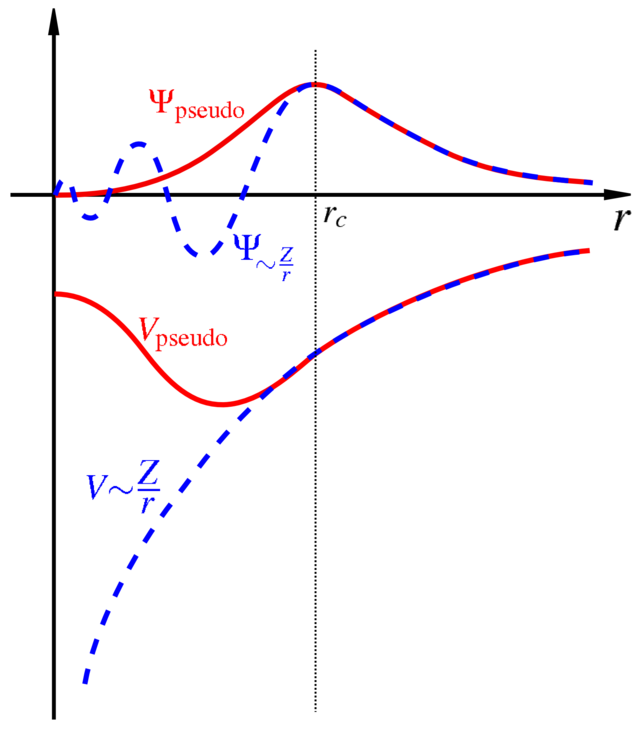
\includegraphics[scale=1.5]{Pseudopotentials.png}
	\caption{Here is an illustration of how a radial cutoff point, $r_c$, is used in a pseudopotential theory to separate the pseudowavefunction into a part that agrees well with the true wavefunction and a section which is only an approximation.}
	\end{figure}

	There are multiple sets of pseudopotentials that the solid state community uses.  They are found via a combination of experiment and calculation, and their accuracy is improving with time\citealp{planewave}.  
	
	\begin{thebibliography}{5}
	
	\bibitem{solidstate} Walter A. Harrison, \textsl{Solid State Theory} (Dover Publications, Inc., 1980)

	\bibitem{electronic} Richard Martin, \textsl{Electronic Structure} (Cambridge University Press, 2004)

	\bibitem{nanosolids} Frank J. Owens \& Charles P. Poole, Jr., \textsl{The Physics and Chemistry of Nanosolids} (John Wiley \& Sons, Inc., 2008)

	\bibitem{convergence} C. Yang, \textsl{On the Convergence of the Self-Consistent Field Iteration for a Class of Nonlinear Eigenvalue Problems} (SIAM, 2009)
	
	\bibitem{planewave} J. Shepherd, \textsl{Convergence of many-body wavefunction expansions using a plane wave basis: from the homogeneous electron gas to the solid state} (Phys. Rev. B, 2012)
	
	\end{thebibliography}
	
\end{document}

